
\kapitel{Using SRI}
\thispagestyle{plain}
\renewcommand\section{\stdsection}
\setcounter{section}{4}
\subsection{Starting SRI}
Open Windows PowerShell as administrator:

\begin{figure}[H]
    \centering
    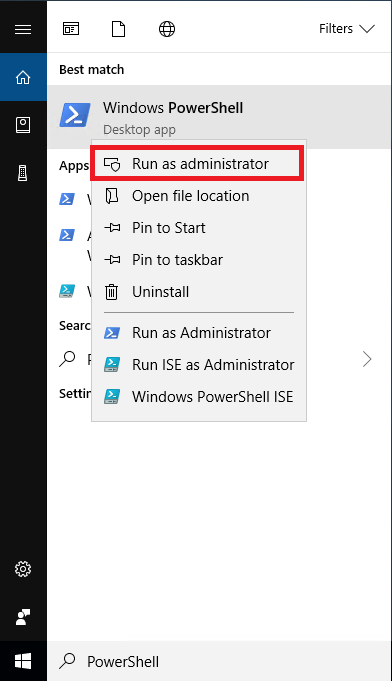
\includegraphics[width=0.35\linewidth]{assets/ps_admin.png}
    \caption{Open PowerShell as Administrator}
\end{figure} \ \\
Navigate to the path the SRI is saved:
\begin{figure}[H]
    \centering
    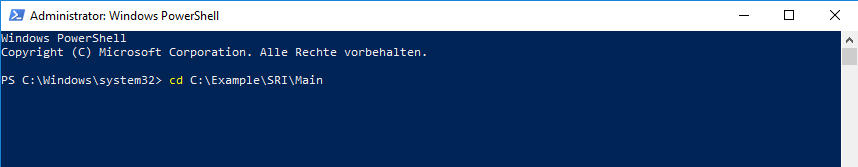
\includegraphics[width=1\linewidth]{assets/open_sri.png}
    \caption{Navigate to SRI}
\end{figure} \ \\
PowerShell is by default not allowed to run scripts. We have to change that to be able to run the SRI. Enter the command ''PowerShell -Exec Bypass''.
\begin{figure}[H]
    \centering
    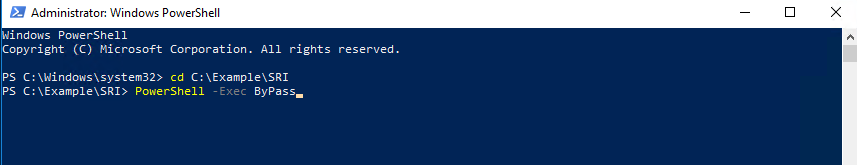
\includegraphics[width=1\linewidth]{assets/ps_bypass.png}
    \caption{PowerShell Bypass}
\end{figure} \ \\
Now you can run the SRI by open the sri.ps1 file. You find more details to the different modes in the section below.
\begin{figure}[H]
    \centering
    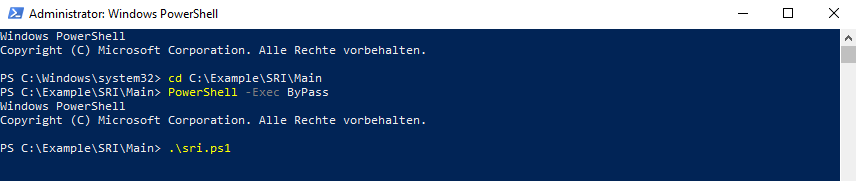
\includegraphics[width=1\linewidth]{assets/sri_ps1.png}
    \caption{PowerShell Bypass}
\end{figure} \ \\

\subsection{SRI modes}
As described in \nameref{GeneralInfo} there are four different modes to run the SRI. These modes are described more precisely in this chapter. These are the four modes:
\begin{itemize}
    \item \textbf{\textit{-Online, -Offline, -GroupPolicy and -AllGroupPolicies}}
\end{itemize}
\begin{lstlisting}[caption=]
PS C:\>./sri.ps1 [-Online] [-OnlineExportPath <String>] [-CAPI2LogSize <Int32>]

PS C:\>./sri.ps1 [-Offline] [[-AuditPolicies]] [[-EventLogs]] [-ImportPath] <String> 
                       [[-ExportPath] <String>] [-CAPI2LogSize <Int32>]

PS C:\>./sri.ps1 [-GroupPolicy] [-GroupPolicyName] <String>

PS C:\>./sri.ps1 [-AllGroupPolicies]
\end{lstlisting}

\vspace{0.5cm}
\textsc{\textbf{Note:}}\textit{ Mandatory parameter are \underline{underlined}.}
\vspace{0.5cm}

\clearpage
The parameters ''-OnlineExportPath'', ''-ImportPath'' and ''-ExportPath'' are Strings, for example:\ \\
\begin{lstlisting}[caption=]
    "C:\Example\Path"
\end{lstlisting} \ \\
The parameters ''-CAPI2LogSize'' is a Integer, for example:\ \\
\begin{lstlisting}[caption=]
    4194304
\end{lstlisting}
The parameters ''-GroupPolicyName'' is a String, for example:\ \\
\begin{lstlisting}[caption=]
    "Default Domain Policy"
\end{lstlisting}

\subsubsection{Online Mode}

\begin{tcolorbox}
    \paragraph{\underline{-Online}} \ \\\\
    The current system which is calling the script will be checked on its readiness.
    \vspace{0.3cm}
    \begin{center}
        \textsc{Parameter}
    \end{center}
    \vspace{-0.5cm}
    \begin{table}[H]
        \def\arraystretch{2}
        \centering
        \begin{tabular}{ p{4cm}  p{10cm} }  \hline
            \textbf{No parameter} & The result PDF will be saved to the current path \\ \hline
            \textbf{-OnlineExportPath} & The result PDF will be saved to this path \\ \hline
            \textbf{-CAPI2LogSize} & Definition of the CAPI2 log size suitable for the environment. By default this value is set to 4MB as recommended from Microsoft  \\ \hline
        \end{tabular}
    \end{table}
\end{tcolorbox} \ \\
These are all possible parameter combinations for the -Online mode: \ \\
\begin{lstlisting}[caption=]
    .\sri.ps1 -Online	

    .\sri.ps1 -Online -CAPI2LogSize 4194304

    .\sri.ps1 -Online -OnlineExportPath "C:\temp\test\targetpath"

    .\sri.ps1 -Online -OnlineExportPath "C:\temp\test\targetpath" -CAPI2LogSize 4194304
\end{lstlisting}

\subsubsection{Offline Mode}

\begin{tcolorbox}
    \paragraph{\underline{-Offline}} \ \\\\ Some system will be checked on its readiness - by default audit policies and event log are analysed. Export files of this system are required.
    \vspace{0.3cm}
    \begin{center}
        \textsc{Parameter}
    \end{center}
    \vspace{-0.5cm}
    \begin{table}[H]
        \def\arraystretch{2}
        \centering
        \begin{tabular}{ p{4cm}  p{10cm} }  \hline
            \textbf{\underline{-ImportPath}} & Defines where the required files rsop.xml\footnote{XML-Export of Resultant Set of Policy}, windowslogs.csv\footnote{Export of Windows logs ''System'' \& ''Security'' from EventViewer, check example\_windowslogs.csv}, appandservlogs.csv\footnote{Export of Application and Service logs ''TaskScheduler'', ''WindowsRemoteManagement''and \ \\ ''LocalSessionManager'' from EventViewer, check example\_appandservlogs.csv} remain for analysis. \\ 
            & The result PDF will be saved to the current path \\ \hline
            \textbf{-AuditPolicies} & Checks only the audit policies. \\
            & The result PDF will be saved to the current path \\ 
            & \textbf{\underline{-ImportPath}} requires rsop.xml \\\hline
            \textbf{-EventLogs} & Checks only the event logs \\
            & The result PDF will be saved to the current path \\ 
            & \textbf{\underline{-ImportPath}} requires windowslogs.csv and appandservlogs.csv\\\hline
            \textbf{-ExportPath} & The result PDF will be saved to this path \\ \hline
            \textbf{-CAPI2LogSize} & Definition of the CAPI2 log size suitable for the environment. By default this value is set to 4MB as recommended from Microsoft  \\ \hline
        \end{tabular}
    \end{table}
\end{tcolorbox}

\clearpage

These are all possible parameter combinations for the -Offline mode: \ \\
\begin{lstlisting}[caption=]
    .\sri.ps1 -Offline -ImportPath "C:\temp\test"

    .\sri.ps1 -Offline -ImportPath "C:\temp\test" -CAPI2LogSize 4194304
    
    .\sri.ps1 -Offline -ImportPath "C:\temp\test" -ExportPath "C:\temp\test\targetpath"
    
    .\sri.ps1 -Offline -ImportPath "C:\temp\test" -ExportPath "C:\temp\test\targetpath" -CAPI2LogSize 4194304
    
    .\sri.ps1 -Offline -EventLogs -ImportPath "C:\temp\test"
    
    .\sri.ps1 -Offline -EventLogs -ImportPath "C:\temp\test" -ExportPath "C:\temp\test\targetpath"
    
    .\sri.ps1 -Offline -AuditPolicies -ImportPath "C:\temp\test"
    
    .\sri.ps1 -Offline -AuditPolicies -ImportPath "C:\temp\test" -CAPI2LogSize 4194304
    
    .\sri.ps1 -Offline -AuditPolicies -ImportPath "C:\temp\test" -ExportPath "C:\temp\test\targetpath"
    
    .\sri.ps1 -Offline -AuditPolicies -ImportPath "C:\temp\test" -ExportPath "C:\temp\test\targetpath" -CAPI2LogSize 4194304
\end{lstlisting}

\clearpage

\subsubsection{GroupPolicy Mode}

\begin{tcolorbox}
    \paragraph{\underline{-GroupPolicy}} \ \\\\ Audit policies from a specific group policy are analysed.
    \vspace{0.3cm}
    \begin{center}
        \textsc{Parameter}
    \end{center}
    \vspace{-0.5cm}
    \begin{table}[H]
        \def\arraystretch{2}
        \centering
        \begin{tabular}{ p{4cm}  p{10cm} } \hline
            \textbf{\underline{-GroupPolicyName}} & The name of the group policy to be analysed \\ \hline
        \end{tabular}
    \end{table}
\end{tcolorbox}\ \\
These is an example for the -GroupPolicy mode: \ \\
\begin{lstlisting}[caption=]
    .\sri.ps1 -GroupPolicy -GroupPolicyName "Default Domain Policy"
\end{lstlisting}\ \\

\subsubsection{AllGroupPolicies Mode}

\begin{tcolorbox}
    \paragraph{\underline{-AllGroupPolicies}} \ \\\\
    All audit policies from every group policy in the current domain are analysed.\\
    The result PDF will be saved to the current path
\end{tcolorbox}\ \\
These is an example for the -GroupPolicy mode: \ \\
\begin{lstlisting}[caption=]
    .\sri.ps1 -AllGroupPolicies
\end{lstlisting}
